\documentclass[14pt,a4paper,oneside]{article}

\usepackage[utf8]{inputenc}   


\usepackage{amsmath,amsthm,amssymb,appendix,bm,mathrsfs,ctex,geometry,tcolorbox,fancyhdr,tikz,esint,appendix}


%% GB/T 7714 宏包 ---- 引文格式
\usepackage[sort&compress]{gbt7714}
\bibliographystyle{gbt7714-numerical}



\numberwithin{equation}{subsection}             %%%%%% 公式编号




\geometry{left=1.7cm, right=1.7cm, top=2.54cm, bottom=2.54cm}    %%%%% 页面尺寸
\linespread{1.5}                             %%%%% 行距1.5倍
\pagestyle{fancy}



%%    设置页眉页脚
\fancyhf{}
\renewcommand{\headrulewidth}{0.15mm}
\fancyhead[C]{文献阅读报告}                   %%%%%% 页眉
\fancyfoot[C]{\thepage}                      %%%%%% 页脚 页码
\setlength{\headheight}{15pt}


%%   设置各种链接颜色为黑色
\usepackage[colorlinks,
            linkcolor=black,
            anchorcolor=black,
            citecolor=black,
            urlcolor=black
            ]{hyperref}



%%   例子编号
\newcounter{example}
\counterwithin{example}{subsection}
\newcommand{\examplename}{Example}
\newcommand{\exampleTitle}[1]{%
\textbf{\refstepcounter{example}\examplename\theexample:#1}\par}


%%  插入图片配置
\usepackage{graphicx,subfigure}
\usepackage[]{caption2} %新增调用的宏包
\numberwithin{figure}{subsection}               %%%%%% 图片编号

\graphicspath{ {./Figure/} }            %%%%% 设置图片文件所在目录
\DeclareGraphicsExtensions{.pdf,.svg,.jpeg,.png,.jpg}     %%%%% 支持图片格式


%%    支持tikz作图
\usepackage{tikz}
\usetikzlibrary{backgrounds,arrows}


\usepackage{pgfplots}
\pgfplotsset{compat=1.15}
\usepackage{mathrsfs}


\title{\textbf{文献阅读报告 5\\Nonlinear pulse compression in a multi-pass cell}}                           %%%%% 标题
\author{骆禹天}                                           %%%%% 作者
\date{2024/**/**}                                        %%%%%% 日期

%%   定义一些数学格式
\newtheorem{theorem}{定理}[subsection]
\newtheorem{definition}[theorem]{定义}
\newtheorem{lemma}[theorem]{引理}
\newtheorem{corollary}[theorem]{推论}
\newtheorem{example}[theorem]{例}
\newtheorem{proposition}[theorem]{命题}
\renewcommand{\abstractname}{\Large\textbf{摘要}}




%------------------------- 开始文档  -------------------------%



\begin{document}

\pagenumbering{Roman}         %%%%% 目录前页码统计按罗马数字

\maketitle

\setcounter{page}{1}          %%%%% 标题开始统计页数

%------------------------- 目录  ------------------------------%

\tableofcontents              %%%%% 插入目录

\newpage                      
\setcounter{page}{1}          %%%%% 目录后重新统计页数


\pagenumbering{arabic}        %%%%% 目录后统计页码为阿拉伯数字



%%%%%%%%%%%%%%%%%%%% 开始第一节  %%%%%%%%%%%%%%%%%%%%%



\section{Introduction}

\subsection{超快光学在材料加工领域需求}

1. 最大化工业微加工应用的效率和吞吐量, 需要高平均输出功率以及 10-100 $\mathrm{\mu J}$ 的脉冲能量. 

2. 更短脉冲利于提高精度以及实现基于多光子吸收或成丝的新颖制造机制\cite{kiselevFilamentinducedLaserMachining2010, gattassFemtosecondLaserMicromachining2008}. 

需求: 基于 Yb:YAG 和掺镱光纤已实现平均功率数百瓦的超快激光器, 但受限于激光介质的增益带宽, 激光脉冲持续时间仅数百飞秒. 



\subsection{产生更短脉冲方法: 非线性脉冲压缩} 

当脉冲通过 $\chi^{(3)}$ 非线性介质时, 由于光克尔效应导致的自相位调制 (SPM), 脉冲光谱展宽. 抵消展宽脉冲的啁啾后, 可获得时间压缩脉冲. 

由于克尔效应的空间作用, SPM 伴随自聚焦, 导致光束质量下降. 且若峰值功率超过材料阈值会发生破坏性的自聚焦. 

非线性介质:

· 电介质 (常用熔融石英) : 受到自聚焦限制, 熔融石英中自聚焦发生在线性偏振光的峰值功率约 4 MW 时. 迄今电介质非线性压缩最高平均功率为 250 W (23 fs 压缩脉冲持续时间, 69\% 压缩效率) , 使用无源大模场面积光子晶体光纤\cite{jocherSub25Fs2012}. 

· 惰性气体: 压缩较高能量脉冲, 自聚焦阈值高约三个量级. 多数实验在充气空心毛细管中进行. 由于毛细管的非线性度显着降低且实际尺寸较大, 该方法在持续时间为 100 fs 的输入脉冲的情况下通常用于输入脉冲能量超过 100 $\mathrm{\mu J}$ 情形. 使用这种方法压缩的最高平均功率为 400 W (<30 fs 输出脉冲持续时间, 58\% 压缩效率, ~300 $\mathrm{\mu J}$ 脉冲能量) \cite{hadrich200AveragePower2016}. 

上述方案在脉冲能量 10-100 $\mathrm{\mu J}$ 范围留下了间隙 (对于亚 ps 输入脉冲) , 两种脉冲压缩方案都不可行. 近年来, 人们付出努力希望缩小基于稀有气体方案的脉冲能量或者增大基于电介质方案的脉冲能量. 

对前者, 可使用充气空心 Kagome 光子晶体光纤. \cite{emauryEfficientSpectralBroadening2014, guichardNonlinearCompressionHigh2015, hadrichExploringNewAvenues2015} 目前已经实现 118 W 输出功率下的光谱展宽 (在 8.4\% 的功率下压缩至88 fs, 输出脉冲能量 18 $\mathrm{\mu J}$) \cite{emauryEfficientSpectralBroadening2014}. 在另一实验中, 压脉冲至 31 fs, $\sim$80\%的压缩效率, 输出功率为 76 W (7 $\mathrm{\mu J}$ 输出能量) \cite{hadrichExploringNewAvenues2015}. 这些结果表明充气空心 Kagome 光子晶体光纤的平均功率可扩展性. 

\begin{figure}[h]
    \centering
    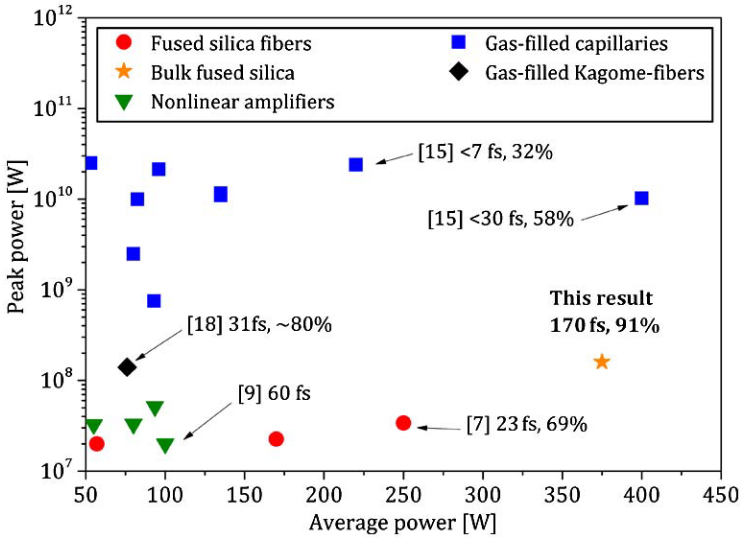
\includegraphics[width=0.4\textwidth]{p1.png}
    \caption{包含非线性脉冲压缩的高功率激光系统 (>50 W) 概述}\label{p1.2.1}
\end{figure}

对后者, 引入了多路展宽的概念：光谱展宽前, 脉冲分成几个峰值功率低于自聚焦阈值的副本, 在非线性介质之后再相干地组合\cite{guichardEnergyScalingNonlinear2013, klenkeCoherentCombinationSpectrally2014}. 已实现压缩 7.5  脉冲 (71 fs 脉冲持续时间, 750 mW 平均输出功率) \cite{klenkeCoherentCombinationSpectrally2014}, 但该方法的平均功率可扩展性尚未得到证实. 

另外, 可用单个块体电介质取代在波导中进行光谱展宽压缩超过自聚焦阈值的脉冲\cite{rollandCompressionHighpowerOptical}. 这种情况, 介质的长度及输入光束直径和发散度需精确调节, 以避免自聚焦. 实验上, 已经实现在平均输入功率为 50 W、脉冲能量为 1.38 $\mathrm{\mu J}$ 时将 250 fs 脉冲压缩到 43 fs , 但该方案由于空间克尔效应的作用, 需要空间滤波, 且本质上压缩效率限制在$\sim$60\%\cite{seidelAllSolidstateSpectral2016}. 

\subsection{作者工作的总结与意义}

(1) 基于块体电介质, 10-100 $\mathrm{\mu J}$ 范围脉冲压缩:

· 减轻了单一体介质中光谱展宽的缺点, 

· 稳健性,

· 平均功率缩放能力.

(2) 利用多通腔 (MPC) 在非线性介质薄片中来回传输, 每次传输对应 B 积分 $\ll \pi$, 非线性相位在多次通过期间累积, 因此可以实现总 B 积分 $>4\pi$ 和显著的光谱展宽:

· 峰值功率高于自聚焦阈值的光谱展宽,

· 减轻穿过非线性介质时光束质量的下降,

· MPC 可以设计使其具足够的通光孔径, 以使MPC对输入光束的对准、指向和光束质量不敏感. 

(3) MPC的潜在限制:

除 MPC 尺寸限制, 仅受到激光引起非线性介质、MPC 光学器件及其镀层损坏的限制. 该方法使用抗反射 (AR) 镀层熔融石英作为非线性介质, 并使用电介质镀层反射镜作为 MPC 和压缩光学器件, 适合平均功率为 kW 级的超快激光源的脉冲压缩. 

\section{Set up}

\subsection{MPC}

· 两个曲率 $\pm 350$ mm、直径 50 mm 透镜.

· 凹面朝向 MPC 的中心涂有增透膜, 凸面涂有高反射 (HR) 膜. 这样, 镜基片就可以作为非线性介质. 

· 厚度为 13 mm 的熔融石英基底. 为了补偿基底材料色散, HR 镜面镀层具有每次反射 GDD 为 $-400 \pm100 \mathrm{fs^2}$ 的色散. 镜距选择为$\sim$540 mm, 即无克尔透镜的情况下该模式在曲面镜处的光束半径为460 $\mathrm{\mu m}$. 

· 两个直角熔融石英棱镜放置在 MPC 相对侧靠近 MPC 反射镜的位置将光束耦合进出 MPC. 调节耦合镜, 使光斑分布在腔镜上呈圆形. 

· 38 通, 非线性介质中总传播长度 $\sim1$ m, 自由空间中总传播长度 $\sim20$ m

\begin{figure}[h]
    \centering
    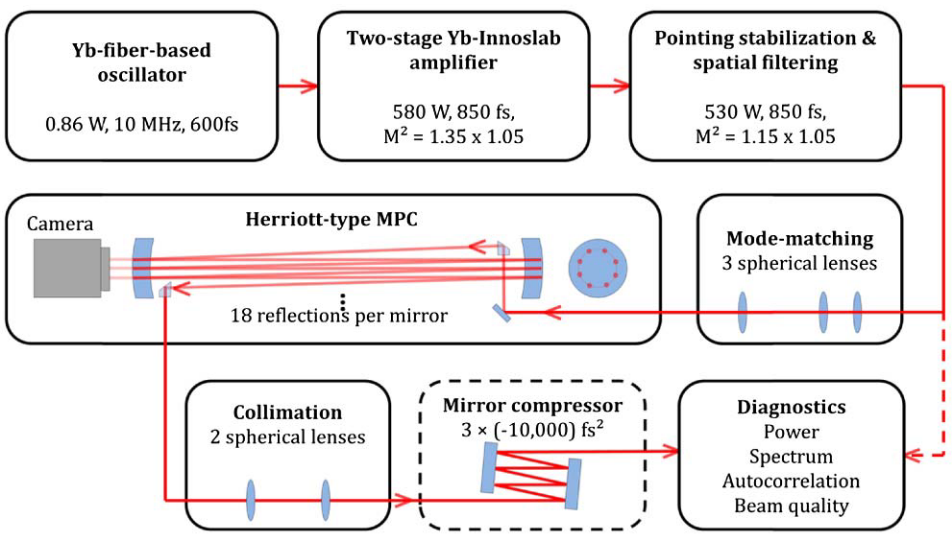
\includegraphics[width=0.6\textwidth]{p2.png}
    \caption{多通腔非线性压缩实验装置}\label{p2.1.1}
\end{figure}

\subsection{Input}

· 两级 Yb:YAG-Innoslab 放大器系统, 该系统由商用掺镱光纤振荡器提供种子, 包括一个空间滤波模块, 以提高光束质量\cite{russbueldtInnoslabAmplifiers2015}

· 该系统在重复频率 10 MHz 下提供高达 530 W 的输出功率, 脉冲持续时间为 850 fs (FWHM 带宽 1.6 nm) , 光束质量几乎受到衍射限制 ($M^2_X \times M^2_Y =1.17 \times 1.05$) . 

\subsection{Mode Match}

· 3个球面透镜. 光束从其中一个 MPC 反射镜透射被成像到相机, 从而可测量每次往返后的光束半径以优化模式匹配, 

· 光束耦合出 MPC 后, 用2个球面透镜准直. 通过光圈, 可将输出光束与 MPC 反射镜镀增透膜表面的残余反射分离开. 

%--------------------  第三节 结果  --------------------%


\section{Result}

\subsection{总体输出结果}

耦合进 MPC : 平均功率 500 W 和 脉冲能量 50 $\mathrm{\mu J}$,

根据实验确定的最大功率下的光束半径, 估计最大 B 积分为 $\sim5\pi$.  

MPC 的输出功率随输入功率线性增加 [\ref{p3.1.1} (b)], 最大输出功率达446 W. 

总传输效率为91\%, 超过了典型的基于波导光谱展宽的透射率. 

完整的通过MPC 包括 72 次通过 AR 镀膜镜面和 36 次 HR 镀膜镜面反射. 因此, MPC 的损耗主要是由于 MPC 光学器件镀层造成的线性损耗. 

\begin{figure}[h]
    \centering
    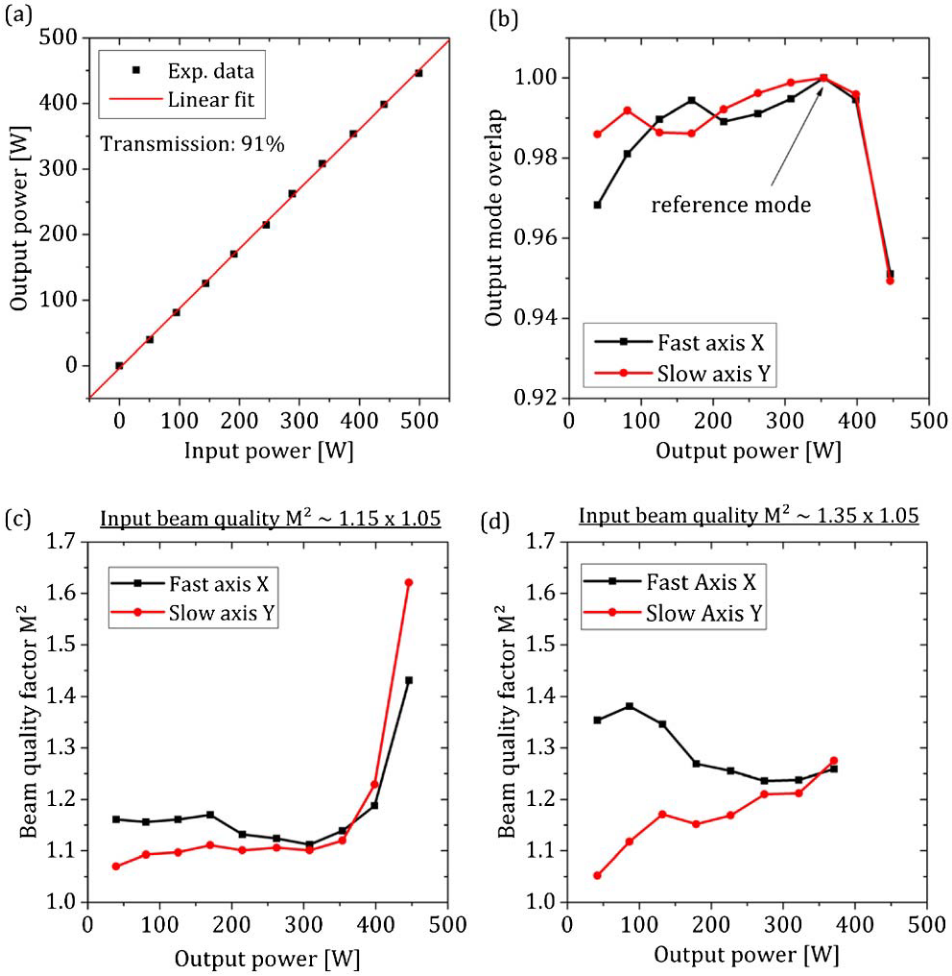
\includegraphics[width=0.5\textwidth]{p3.png}
    \caption{MPC 光谱展宽单元的传输特性: (a) 输出功率与输入功率; (b) 输出模式重叠与输入功率的关系: 输出功率为 354 W 的参考模式; (c) 输出光束质量与输出功率的关系; (d) 输出光束质量与输出功率的关系, 没有对输入光束进行空间滤波 (输入光束质量$\sim1.35 \times 1.05$) . }\label{p3.1.1}
\end{figure}

\subsection{光束质量变化的讨论}

入射到 MPC 的功率可以改变, 无需重新对准 MPC 光束路径. 

两种可能引起光束质量变化的因素:

(1) 克尔透镜: 当改变输入功率时, 模式匹配会发生轻微变化;

(2) 热透镜效应: 可观察到镜子基底局部发热, 这可能由于色散 HR 镀层的吸收. 输入功率约为 500 W 时, 最大温度升高约为 20 K, 并导致热透镜效应, 对模式匹配产生与克尔透镜相当的影响. 

说明: 对于此处介绍的所有测量, MPC 的模式匹配和准直已针对 375 W 的输出功率进行优化且在更改输入功率时不做调整. 

通过测量和拟合焦散, 对 MPC 不同输入功率确定 MPC 准直光学器件后输出的 q 参数. 基于这些 q 参数, 作者计算与在 354 W 输出功率下获得的参考输出模式的模式重叠 [图 \ref{p3.1.1}(b)], 在 MPC 的工作范围内变化小于 6\%. 因此, MPC 输出 q 参数几乎不受非线性元件中 Kerr 透镜效应和热透镜效应的影响. 与单次通过块体非线性介质的光谱展宽相比, 这是一个显着的优势, 其中输出 q 参数强烈依赖于非线性介质中的 B 积分. 

结论: 

(a) MPC 光谱展宽的实验装置基于标准商业光学机械, 可以运行几个小时而无需重新对准. 在 MPC 设置运行几周内, 没有观察到任何 MPC 光学元件的镀层或材料损坏. 

(b) 输出功率高达 $\sim$400 W 时, MPC 输入输出光束质量相差无几 [图 \ref{p3.1.1}(c)]. 但当输出功率提高至 >400 W, 光束质量迅速恶化. 

光束质量受到镜基片中克尔透镜效应和热透镜效应产生的像差的影响, 假设不同路径通过非线性介质的像差的复杂相加导致输出功率和光束质量之间存在高度非线性依赖. 输出功率为 354 W 时, 测得的光束质量为 $M^2 =1.14 \times 1.12$. 当输出功率向该值增加时, X和Y方向上的波束质量因子同化, 即与MPC输入光束质量相比, X 方向的光束质量因数降低, 而 Y 方向的光束质量因数增加. 这种同化的原因有待进一步调查. 

\subsection{输出光谱表征}

注意: 本文输出光谱的带宽定义为最外侧边沿的光谱强度降至该外侧峰最大强度的一半的点之间的宽度. (由于展宽出现旁瓣)

在 350 W 输出功率下, 光谱带宽为 13.4 nm, 在最大输出功率下达到 16.1 nm 的带宽 (图 \ref{p3.3.1}) . 与放大器 1.6 nm 的输出带宽相比, 增加了 8.4 倍和 10 倍. 带宽的增加与前文估计最大 B 积分的预期相符. 根据测量的光谱, 计算出分别为 160 fs 和 140 fs (FWHM) 的变换极限脉冲持续时间. 

\begin{figure}[h]
    \centering
    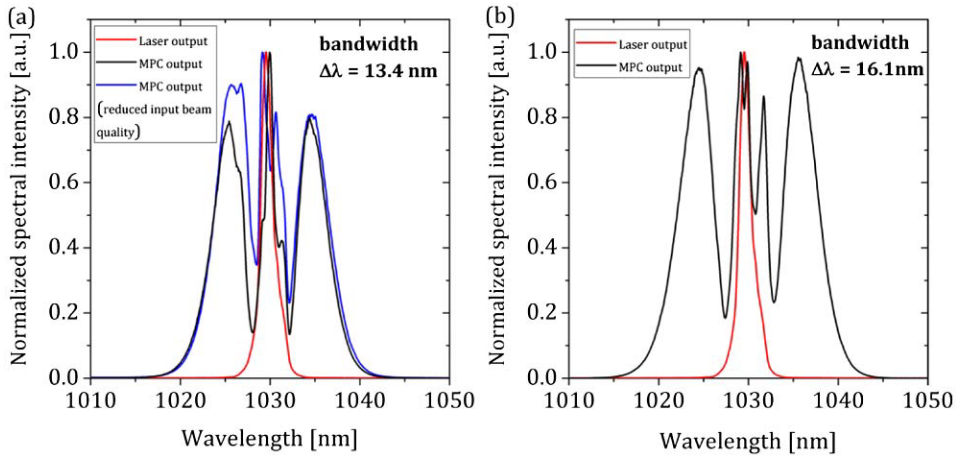
\includegraphics[width=0.6\textwidth]{p4.png}
    \caption{MPC 光谱展宽: (a) 输出功率为 354 W; (b) 最大输出功率 (446 W) 下的输入（红色）和输出（黑色）光谱。 (a) 中的蓝色曲线是在降低输入光束质量的情况下获得的，即在去除激光系统的空间滤波模块后，在输出功率为 370 W 时获得的。}\label{p3.3.1}
\end{figure}

\subsection{分析两种透镜效应对展宽的影响}

为表征光束质量降低时的 MPC 行为, 作者移除 Innoslab 放大器后的空间滤波模块. 

在这种情况下, 入射到 MPC 的光束质量为 $M^2 =1.35 \times 1.05$, 随着输出功率的增加, 观察到 X 和 Y 方向上光束质量的类似同化 [图 \ref{p3.1.1}(d)], 在 370 W 输出功率下产生 $M^2 =1.26 \times 1.28$ 的光束质量. 

在此功率下, MPC 输出的频谱如图 \ref{p3.1.1}(d) 所示. 其 FWHM 带宽与具有空间滤波输入光束的相应光谱的带宽匹配, 这表明: 基于 MPC 的光谱展宽不会敏感地受到输入光束质量的影响. 

\subsection{后压缩与脉冲时域表征}

光谱展宽后通过一个色散镜压缩器将脉冲压缩, 每个啁啾镜(GDD:  $-10000+3000/-8000\;\mathrm{fs^2}$, 带宽: 15 nm) 上三次反射. 

在 375 W 功率和 13.5 nm 带宽下, 观察到最佳压缩效果 [图 \ref{p3.5.1}(a)]. 测得FWHM 宽度为 200 fs, 与变换极限<170 fs匹配. 最终激光系统的脉冲持续时间减少了1/5. 根据自相关曲线, 作者估计约 75\% 脉冲能量包含在主峰中, 对应于估计脉冲能量约 37.5 $\mathrm{\mu J}$ 峰值功率约 160 MW. 

\begin{figure}[h]
    \centering
    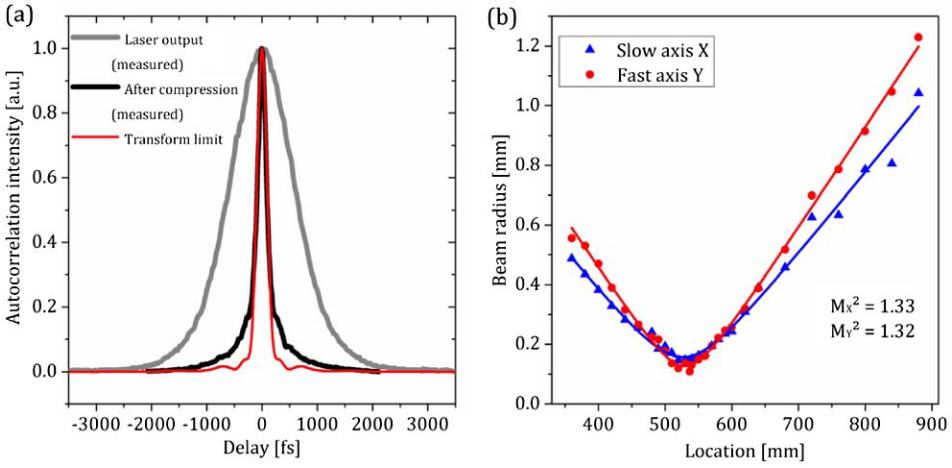
\includegraphics[width=0.5\textwidth]{p5.png}
    \caption{(a) 功率 375 W 压缩后激光输出脉冲的自相关测量以及相应计算的变换极限自相关; (b) 375 W 功率下压缩脉冲后的光束质量测量. }\label{p3.5.1}
\end{figure}

在此功率水平下, 测量压缩器后的光束质量 $M^2= 1.33 \times 1.32$ [图 \ref{p3.5.1}(b)]. 相比图 \ref{p3.1.1}(c) , 光束质量的降低归因于啁啾镜的热效应, 可能由于镀层的吸收. 这提示: 通过降低每次反射的 GDD, 使用具有较低吸收率的压缩器或可提高输出光束质量. 

\section{总结}

有关材料方面的背景介绍;

本文有关MPC的优势的介绍相对完整;

一种相对新颖的MPC配置 ---- 将反射层镀在石英外侧;

虽然似乎两种透镜效应在本文中并不会大幅度影响展宽结果, 但是材料吸收导致的热效应以及空间克尔效应导致光斑质量的下降仍然是值得警醒避免的;

还需要进一步学习有关模场重叠的计算.

%--------------------  插入参考文献  --------------------%

\newpage

\clearpage           %%%  “目录”中显示的页码正确, 需要添加 \clearpage
\phantomsection      %%   “目录”中的链接能正确跳转, 需要添加 \phantomsection
\addcontentsline{toc}{section}{参考文献}   %向目录中添加条目, 以章的名义

\bibliography{ref}

\end{document}